\documentclass{article}

\newcommand\thisclass{CPX 3 Report} % set project/class name

% packages and shortcuts
%% Load additional packages
%\usepackage{keyval} % Used for passing options to packages
%\usepackage{rotating} % Allows for rotation of images
%\usepackage{lettrine} % Used for lettrines
%\usepackage{verbatim} % Allows for verbatim text and block comments
%\usepackage{pdfpages} % Includes pages of finished PDF files
%\usepackage{setspace} % Allows for control of line spacing
%
% Typeset SI units per ISO standard
%\usepackage[load-configurations = abbreviations,
%            per-mode = symbol,
%            inter-unit-separator = {}\cdot{},
%            mode = math]{siunitx}

\usepackage{amssymb}
\usepackage{amsmath}
%\usepackage{amsthm}
%\usepackage{appendix}
\usepackage{array}
%\usepackage[style=numeric]{biblatex}
%\addbibresource{example.bib}
\usepackage{asymptote}
\usepackage{bytefield}
\usepackage{cancel}
\usepackage{changepage}
\usepackage[american]{circuitikz}
%\usepackage{cite}
\usepackage{colortbl}
\usepackage{comment}
%\usepackage{coloremoji}
\usepackage{empheq}
%\usepackage{enumerate}
\usepackage{enumitem}
%\usepackage{esint}
\usepackage{etoolbox}
\usepackage{fancyhdr}
%\usepackage{filecontents}
\usepackage{float}
\usepackage{hanging}
%\usepackage{nomencl}
%\usepackage{fancyref}
\usepackage[margin=1in, bottom=1in]{geometry}                
\usepackage{lastpage}
%\usepackage{listings}
\usepackage{mathabx}
\usepackage{mathrsfs}
\usepackage{mathtools}
%\usepackage{multicol}
%\usepackage{multido}
\usepackage{multirow}
\usepackage{pbox}
\usepackage{pgf}
\usepackage{pgfplots}
\pgfplotsset{compat=1.18}
%\usepackage{pgf-pie}
\usepackage{pgfplotstable} 
%\usepackage{pgfcalendar}
\usepackage{pdflscape}
\usepackage{pdfpages}
%\usepackage{pgfgantt}
\usepackage{ragged2e}
\usepackage{steinmetz}
%\usepackage{subfig}
\usepackage{subcaption}
\usepackage{textcomp}
\usepackage{tikz}
\usepackage{tkz-euclide}
\usepackage{tikzducks}
\usepackage{tikzscale}
\usetikzlibrary{decorations.pathmorphing, ducks}
\usepackage[absolute,overlay]{textpos}
\usetikzlibrary{calc}
\usetikzlibrary{decorations.markings,positioning,arrows,shapes,patterns}
%\usepackage{./LaTeX/3dplot}
\usetikzlibrary{calc}
\usepackage{tikz-3dplot}
\usetikzlibrary{arrows}
%\usepackage{titling}
\usepackage{wrapfig}
\usepackage{varioref}
\usepackage[x11names]{xcolor}
%\usepackage{../../tools/matlab/mcode}
%\usepackage{slashbox}

% page formatting
%\geometry{letterpaper}                   % ... or a4paper or a5paper or ... 
%\geometry{landscape}                % Activate for for rotated page geometry
%\usepackage[parfill]{parskip}    % Activate to begin paragraphs with an empty line rather than an indent

\usepackage{graphicx}
%\usepackage{animate}

\usepackage{longtable}
\usepackage{booktabs}
\usepackage{pdflscape}

\usepackage{listings}
\usepackage{xcolor}

\let\degree\relax
\usepackage{gensymb}
\usepackage[none]{hyphenat}

%%%%%%%%%%%%%% Packages %%%%%%%%%%%%%%%%

\usepackage[colorlinks=true,
    linkcolor=blue,hidelinks]{hyperref}
\usepackage{endnotes}

%%%%%%%%%%%%%% Page Formating %%%%%%%%%%%%%
\setlength{\parskip}{1em} % add packages here
% Custom Commands
\def\unit#1{\, \text{#1} \, }
\def\code#1{\texttt{#1}}


% Custom Colors
\definecolor{myblue}{RGB}{0,119,187}
\definecolor{myred}{RGB}{187,85,102}
\definecolor{mycyan}{RGB}{51,187,238}
\definecolor{myteal}{RGB}{0,153,136}
\definecolor{myorange}{RGB}{238,119,51}
\definecolor{mymagenta}{RGB}{238,51,119}
\definecolor{mygrey}{RGB}{187,187,187}
\definecolor{lightcyan}{rgb}{0.84,1,1}
\definecolor{lightgreen}{rgb}{0.64,1,0.71}
\definecolor{lightred}{rgb}{1,0.7,0.71}
\def\myred{red!65!black}  % these are custom shortcuts


% page options
\pagestyle{fancy}
\setlength\parindent{0pt}
\addtolength{\textheight}{-18pt}
\fancyhead{}
\fancyfoot[L]{\thisclass}
\fancyfoot[R]{\thepage}
\fancyfoot[C]{}
\renewcommand{\headrulewidth}{0pt}
\renewcommand{\footrulewidth}{1pt}






% DOCUMENT STARTS HERE

\begin{document}
	

% Title Page
\hypersetup{pageanchor=false} % so the title page and front matter don't try to act like page 1 of the document later...

\begin{center}

\includegraphics[scale=0.25]{./figures/ECE-logo.png} \\[24pt]
\huge{\textbf{\thisclass}} \\[12pt]
\Large{ECE 434: Digital Signal Processing} \\[4pt]
\Large{\today} \\[4pt]

\vfill

\Large{C1C Victor Chen}

\Large{C1C Ben Cometto}

\Large{C1C Nick Csicsila}

\Large{C1C Geoff Stentiford}
\end{center} 

\newpage


% Table of Contentses
\thispagestyle{empty}
\setcounter{page}{0}
\tableofcontents

\newpage
\listoffigures

\newpage
\listoftables

% Content

\newpage
\hypersetup{pageanchor=true} % re-activate 
% !TEX root =./main.tex


\begin{abstract}

Computer Exercise 2 (CPX 2) required processing 5 signals in a variety of manners to produce certain objectives.  Digital signal processing using various FIR and IIR  filters enabled these objectives to be met with low order filters.  The signals, including test tones, ECG data, and jammed audio, provided a wide range of applications for digital signal processing.  Overall, CPX2 was a great exercise in solving real-world problems using digital filter techniques. 

\end{abstract}

\section{Introduction}

\parindent=0pt
\parskip=.5\baselineskip plus 2pt

Computer Exercise 2 (CPX 2) for ECE 434, Digital Signal Processing, involved processing 5 signals.  The five signals are: 
\begin{itemize}
    \item Signal $x_1$: Two tones, one louder and one softer

    \item Signal $x_8$: A message containing the secrets of sunshine extraction from cucumbers, but important information is jammed

    \item Signal $x_3$: An electrocardiogram (ECG) that is contaminated with a power line artifact

    \item Signal $x_4$: An unknown audio signal that is jammed

    \item Signal $x_7$: A series of 10 test tones that must be modified
\end{itemize}

The processing goals for each signal are:
\begin{itemize}
    \item Signal $x_1$: Make the louder tone softer and the softer tone louder

    \item Signal $x_8$: Reveal the jammed information

    \item Signal $x_3$: Remove the power line artifact

    \item Signal $x_4$: Reveal the unknown audio

    \item Signal $x_7$: Correctly modify the 10 test tones
\end{itemize}

I filtered each signal to enact the signal's processing goal.  All aspects of the filter, including using an infinite impulse response (IIR) versus a finite impulse response (FIR) design method, order, and other parameters, have been carefully considered, and are reported in each signal's respective section.  For access to the Matlab \code{.mlx} files, source signal data, filter designer session \code{.fda} file, filter taps \code{.bin} files, and output \code{.wav} sound files, see the project's GitHub repository at \url{https://github.com/dbcometto/ece434_cpx2}.

 
\newpage
% !TEX root =./main.tex

\section{Block 1: Noise Removal, Bandwidth Limiting, and Bias Correction}

This block carries out three functions: it removes the DC bias inherent to the sensors, reduces the noise
 in the signal, and limits the bandwidth to only that which is needed. This is accompished in three stages:
 preliminary debiasing through the very simple method of subtracting the average value of each sensor channel,
 a high-pass filter to fully remove bias and very low-frequency noise, and a low-pass filter to clamp the
 bandwidth at 20kHz and remove any high-frequency noise. 

\begin{figure}[H]
    \centering
    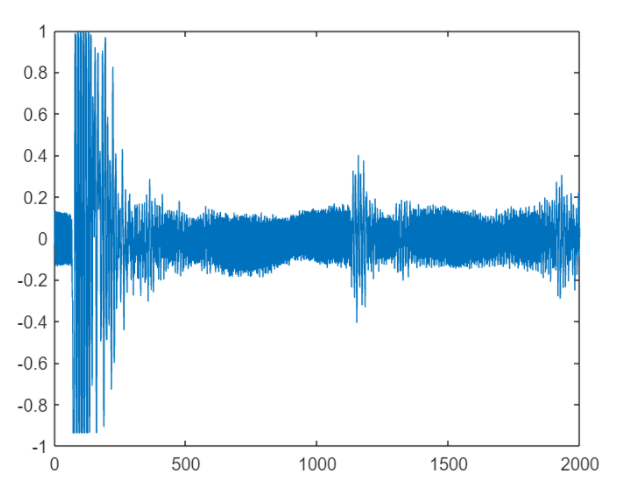
\includegraphics[width=0.5\linewidth]{figures/prefiltered.PNG}
    \caption{Pre-filtered average subtracted only}
\end{figure}
 
The low-pass filter was a 30-order Tukey window filter
with an alpha of 0.5 and a cutoff frequency of 22.16kHz. Its stopband lobes are aligned such that the 25kHz
"jamming" falls directly into one of the cracks. The high-pass filter, meanwhile, is a 61-order least-squares
 filter with a cutoff which targets only the DC component. Using two cascaded filters resulted in a lower total
 order than a single bandpass filter.

\begin{figure}[H]
    \centering
    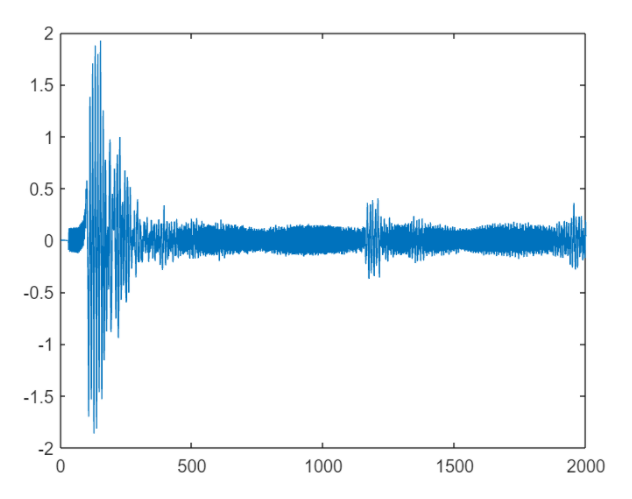
\includegraphics[width=0.5\linewidth]{figures/debiased.PNG}
    \caption{High-pass filtered, DC bias removed}
\end{figure}

An infinite impulse response (IIR) filter, specifically an elliptic filter, would allow for a much lower-order
 filter which would be faster to run, but the need to preserve phase relations meant we restricted ourselves to
 finite impulse response filters to be on the safe side, as FIR filters ensure a linear phase response. Elliptic
 IIR filters do not distort phase too badly, but enough that some amount of distortion is visible in the final
 display.

\begin{figure}[H]
    \centering
    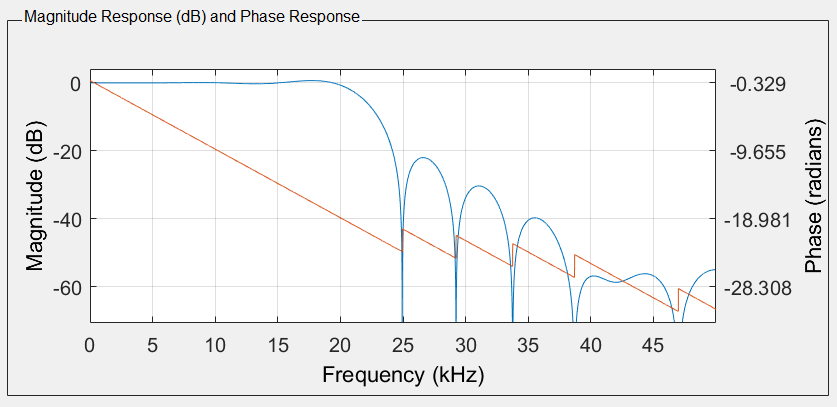
\includegraphics[width=0.5\linewidth]{figures/tukey.PNG}
    \caption{Pre-filtered average subtracted only}
\end{figure}

\begin{figure}[H]
    \centering
    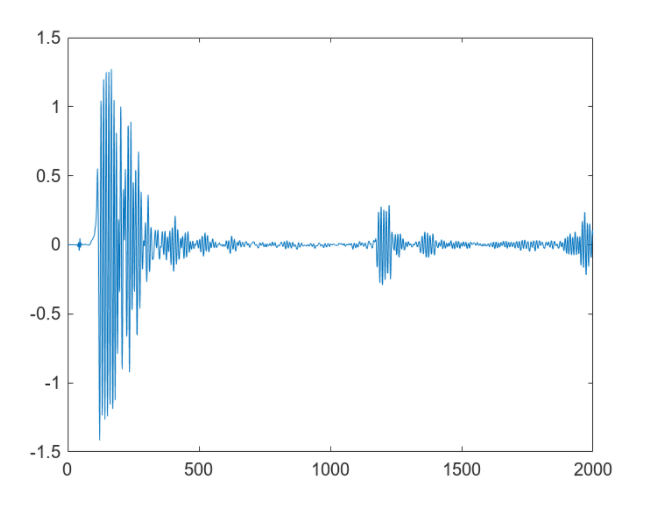
\includegraphics[width=0.5\linewidth]{figures/denoised.PNG}
    \caption{Low-pass filtered, high frequencies removed}
\end{figure}

We decided to place this block first, as the noise-reduced signal is much simpler to deal with when implementing
 the calibration stage than the raw data signal. 
\newpage
% !TEX root =./main.tex

\section{Block 2: Calibration}

The calibration block detects the sonar transmissions, shifts the data in the time domain so that the start
 of the arrays line up with the transmit time, zeros out the transmission, and normalizes the received signal
 across the arrays. To determine where the transmission occurs, the block looks for 10 consecutive samples where
 the absolute value of the signal exceeds 0.08. Then, to determine where it ends, it waits for 30 consective
 samples with a level below 0.04. From there, it shifts the data left to align the array start with the
 transmission's start. To normalize the signal magnitudes, the block examines four signals to find the maximum
 absolute values in each and applies the necessary gain to bring each signal up to the same strength as The
 strongest signal.

To optimize for speed, the calibration stage was made into a unified module instead of a distinct stage 1a and
 stage 1b. By using the already-filtered signal, a much simpler (and therefore faster and less error-prone)
 approach was feasible.  
\newpage
% !TEX root =./main.tex
\section{Block 3 : Time Gain Compensation - Nick Csicsila}

As sound travels, it attenuates through geometric spreading.  As a result, the magnitude of the second reflected pulse is significantly lower. Therefore, the program must compensate to increase the magnitudes of the two pulses back to the original magnitude of 1. 
    The samples must first be converted into distance. This is easily accomplished using the following conversion.
    \begin{align*}
     \frac{\text{Sample Index}}{F_s} \cdot c_{\text{sound}}    
    \end{align*}
    

    Although the speaker has some degree of directivity, the best results were found using the inverse- square law $(I \propto  \frac{1} {r^2} )$. 

    \begin{figure}[H]
        \centering
        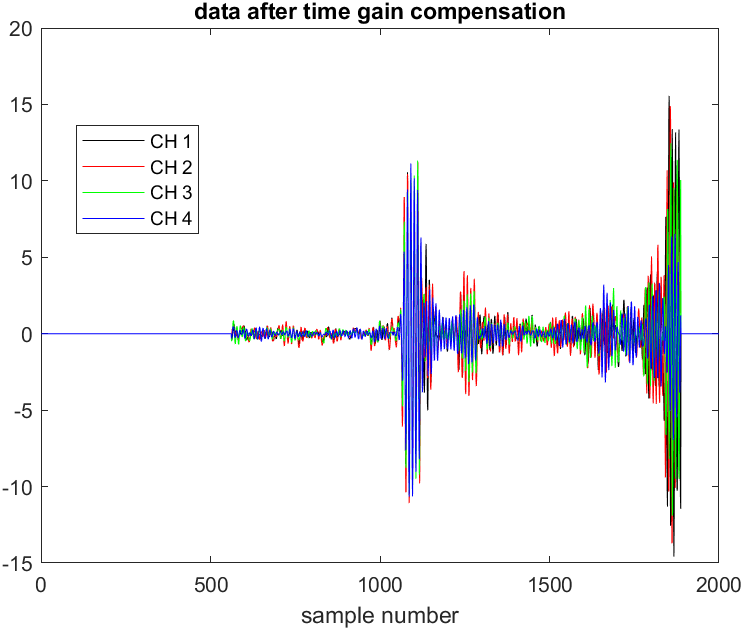
\includegraphics[width=0.5\linewidth]{figures/time_gain_1.png}
        \caption{Data after time gain compensation}
        \label{fig:time_gain1}
    \end{figure}

    \ref{fig:time_gain1}

 
\newpage
% !TEX root =./main.tex

\section{Block 4}
 
\newpage
% !TEX root =./main.tex

\section{Block 5: Beamforming - Victor Chen}

Beamforming is a signal processing technique used to spatially direct signals, enhancing desired signals while suppressing other signals with interference. A delay-and-sum beamforming algorithm is applied to the four-channel system of uniformly spaced linear sensor array of four omnidirectional microphones. Assuming the signal source is in the far field, the incoming wave fronts are approximately linear, enabling the computation of beam angle for each integer sample delay k.

The goal for the beamforming block is to use the delay-and-sum beamforming function 
\begin{align*}
    Beams[k,n] = X_1[n]+X_2[n+k]+X_3[n+2*k]+X+4[n+3*k]
\end{align*}
to spatially focus and enhance signals from a specific direction across our four-channel system.


\subsection{Implementation}

This block is designed to perform beamforming across 4,000 samples from the four channels. Given the need for multiple iterations, it is crucial to balance between processing speed and output quality.

To optimize the beamforming function, we utilize \textsc{MATLAB}'s linear vectorization and precomputing capabilities, enabling faster and more efficient processing by operating on entire data arrays simultaneously instead of relying solely on iterative loops.

\begin{figure}[H]
    \centering
    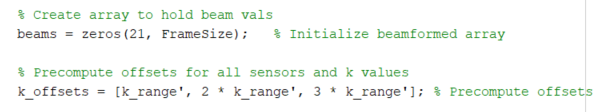
\includegraphics[width=0.5\linewidth]{figures/beamform_fig1.png}
    \caption{Precomuting Equations}
    \label{fig:precomputing_equations}
\end{figure}

The first optimization method involves precomputing the array to store the beams and the offsets for all sensors. This approach preloads the necessary matrices, eliminating the need for dynamic resizing or appending during runtime, which can significantly slow down the program. As illustrated in Figure 1, the k\_offsets for the delays are computed in a single step using vectorized operations. Additionally, a beams array is preallocated in advance to hold the calculated beams, ensuring optimal memory usage and faster processing.

\begin{figure}[H]
    \centering
    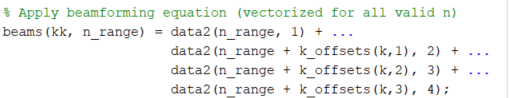
\includegraphics[width=0.5\linewidth]{figures/beamform_fig2.png}
    \caption{Beamforming Computation}
    \label{fig:beamforming_computation}
\end{figure}

The second optimization method involves performing beamforming calculations across all 4,000 samples simultaneously, rather than iterating through each index individually. This reduces the number of loops, making the process much more efficient.



\subsection{Analysis}

After developing the beamforming function, test data was generated to evaluate its performance. The test data consisted of four channels of in-phase sine waves, defined by the equation \textit{sample} = sin(\textit{t}/40), where \textit{t} ranged from 1 to 4,000. After ensuring the function works with the test data, I used data2 directly from the project.

\begin{figure}[H]
    \centering
    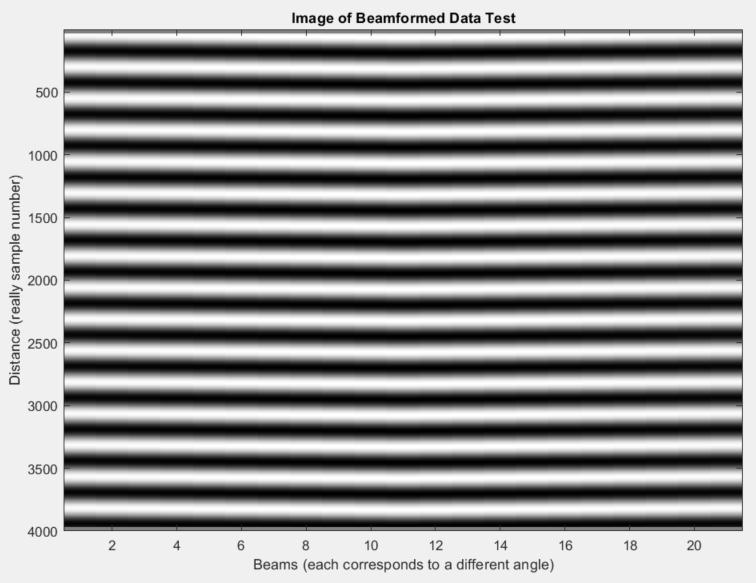
\includegraphics[width=0.5\linewidth]{figures/beamform_fig3.png}
    \caption{Output for Testing with sin(t/40) wave}
    \label{fig:sinwave_output}
\end{figure}

As shown in Figure 3, each black-and-white horizontal line represents a wave. With 4,000 samples in the equation sin(\textit{t}/40), this corresponds to approximately 16 waves. The figure confirms this, demonstrating that the beamforming function performs as expected. It is important to note that the waves are evenly horizontal due to the in-phase channels, however, as the frequency of the waves increases, the evenness of the waves will begin to separate.

\begin{figure}[H]
    \centering
    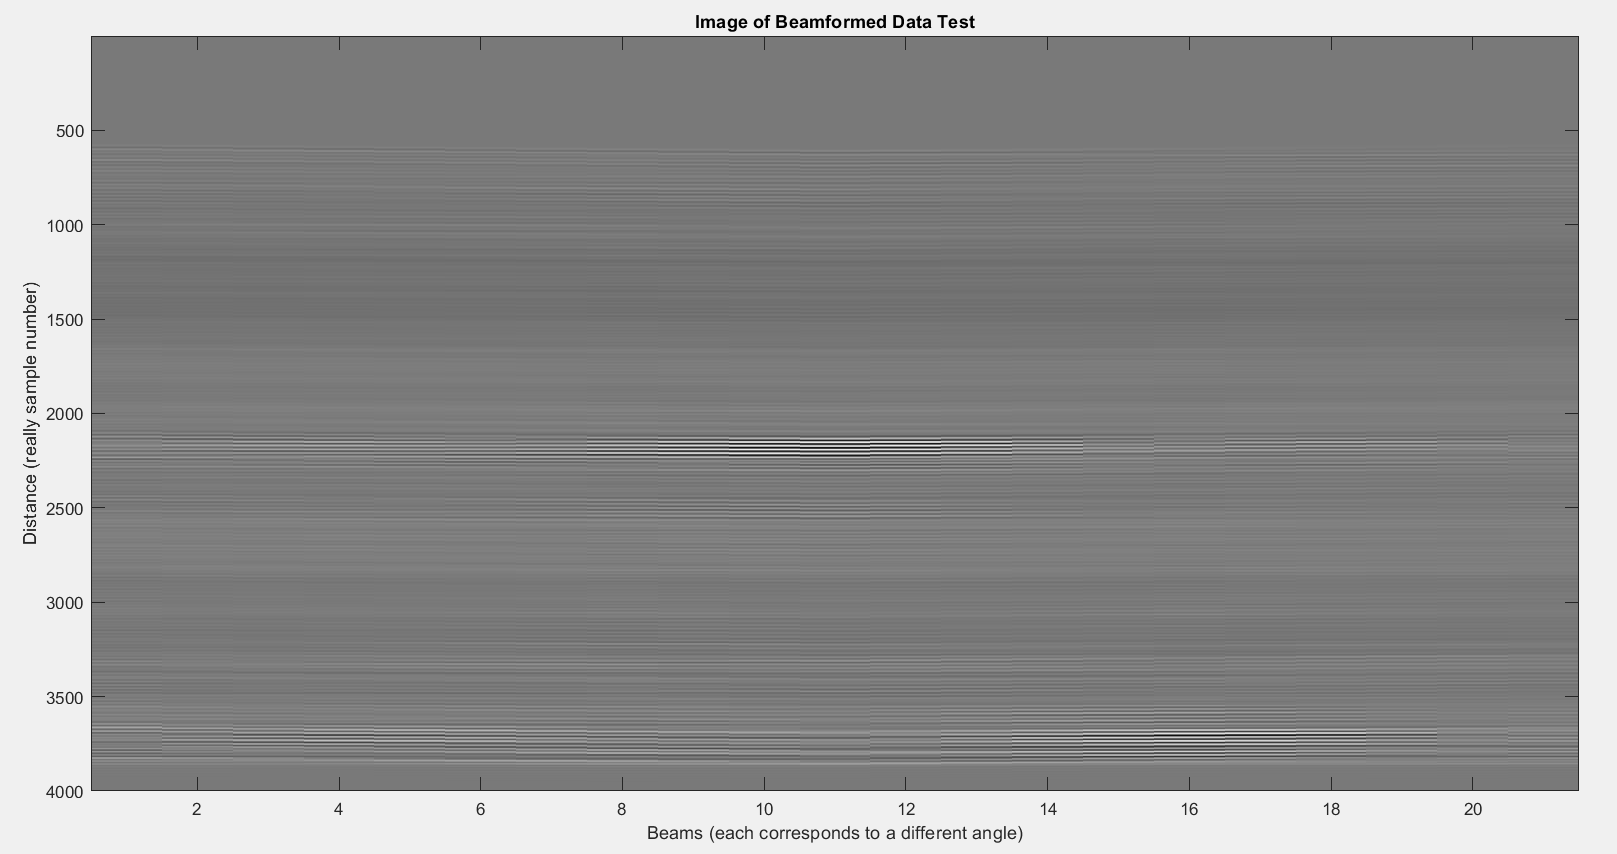
\includegraphics[width=0.5\linewidth]{figures/beamform_fig4.png}
    \caption{Beamform Output from Data}
    \label{fig:final_beamform_output}
\end{figure}

As shown in Figure 4, the beamform output of data2 reveals two regions where the signal strength is highest. These are represented by two prominent white "blobs"--one near the center and another near the bottom-right corner of the beamformed image. These regions indicate areas where the waves return well-constructed, suggesting the presence of an object that the waves interacted with.

\begin{figure}[H]
    \centering
    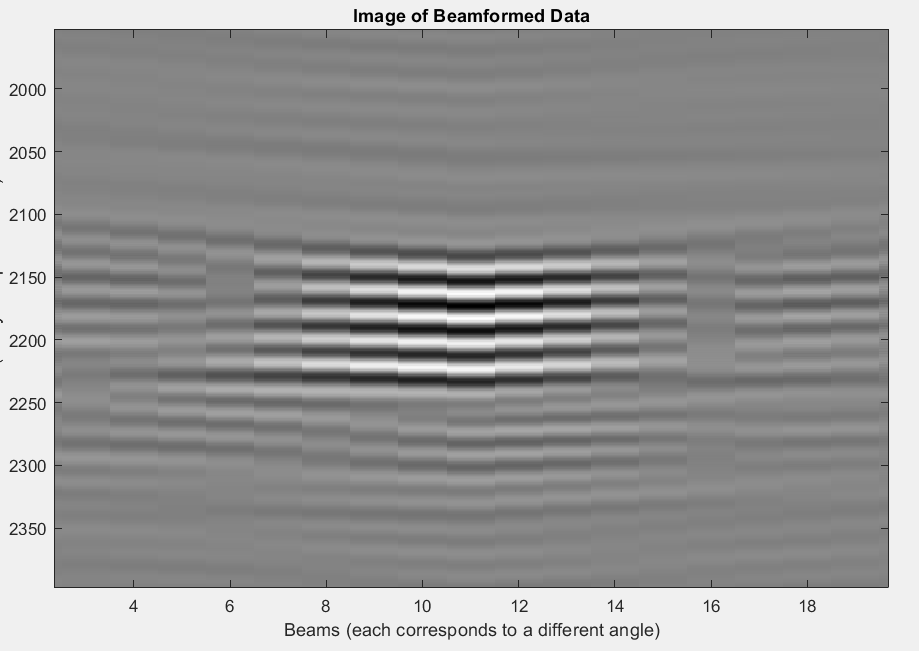
\includegraphics[width=0.5\linewidth]{figures/beamform_fig5.png}
    \caption{Zoomed In Beamform Output}
    \label{fig:zoomed_in_beamform_output}
\end{figure}

By zooming into the center of the beamform image in Figure 5, we can see that while the signal strength is high, each beam is still slightly offset. This offset may be due to inaccuracies in my delay calculations or it might be due to the geometry/spacing of the sensors. Plenty of time was spent on trying to correct the offset by shifting beams, however none were successful. More work will need to be done to correct this issue.


The beamforming function achieved an average execution time of 0.0023155 seconds, a substantial improvement compared to pre-optimization runs, which took tens of seconds. This demonstrates a significant increase in computational efficiency for beamforming.
  
\newpage
% !TEX root =./main.tex

\section{Block 6: Quadrature Demodulation - Chen \& Stentiford}

The quadrature demodulator is used to detect the pulse envelopes. It is a type of 
amplitude modulation (AM) decoder which is able to function without knowing the exact 
phase of the signal's carrier wave. It consists of three stages: mixing, filtering, 
and magnitude calculation.

The mixing stage of a normal (synchronous) demodulator multiplies the received signal 
by the original carrier wave, matching the frequency and phase. Because we do not know 
the phase in this case, we instead split the incoming signal, multipling each copy by 
carrier waves 180° apart. Or, in mathematical terms:

\begin{align*}
    y[n] = x[n]*(\cos(2 \pi f n)+j \cos(2 \pi f n+\pi)) = x[n]*(\cos(2 \pi f n)+j \sin(2 \pi f n))
\end{align*}

To mitigate the relative slowness of trigonometric calculations, we pre-computed a pair of 
tables for cosine and sine which could be used in the actual block instead of calls to 
MATLAB's cosine and sine functions. The tables additionally already account for the sampling 
rate and carrier frequency in order to minimize multiplication operations inside the time-
sensitive block.

After filtering, to merge the imaginary and real components back into a singal envelope, we 
simply take the magnitude:

\begin{align*}
    Y = \sqrt{I^2 + R^2}
\end{align*}

This is achieved as a single-line vector operation, and so is very performant.  
\newpage
% !TEX root =./main.tex

\section{Block 7: Scan Conversion - Cometto}

Scan conversion handles the task of converting the stored beam data (in our case, in Mag\_image) from its polar reference (beam/sample or angle/distance) to a rectangular reference that can be used as data for an image.  Additionally, in order to form a continuous image, the values between the beams must be interpolated.

\subsection{Background}

Before discussing the implementation, we will first discuss the information necessary to understand and accomplish this task.  First, the signal data is stored in an array named \code{Mag\_image} where each row corresponds to a beam (angle), and each column corresponds to a sample (distance).  In our case, the array is $21 \times 4000$.  The output of the scan conversion stage is a $100 \times 201$ pixel image, which will be stored as a $100 \times 201$ array called \code{image}.

We will define the pixel at index $[1,101]$ as our position $(x,y) = (0,0)$.  From there, we can assign each pixel an angle, $\theta_p$, and a distance, $r_p$.  Then, we can perform bilinear interpolation using the equation
\begin{align*}
    \code{image[r,c]} = (1-\beta) &\left( (1 - \alpha) \code{Mag\_image[k,n]} + (\alpha) \code{Mag\_image[k+1,n]}  \right) \\ 
    + (\beta) &\left( (1-\alpha) \code{Mag\_image[k,n+1]} + (\alpha) \code{Mag\_image[k+1,n+1]} \right)
\end{align*}
with
\begin{align*}
    \alpha = \frac{\theta_p - \theta_k}{\theta_{k+1} - \theta_k}
\end{align*}
and
\begin{align*}
    \beta = \frac{r_p - r_n}{r_{n+1} - r_n}
\end{align*}
as the fractional offsets in the angle and distance directions, respectively.  This allows us to use use a weighted average of the four nearest known values to calculate the value at every pixel of the output image.

\subsection{Implementation}

In order to implement this algorithm in a fast way, we need to precompute as much as possible.  With the right values precomputed, it is possible to completely vectorize the function, as is done in \code{scan\_conversion.m}.  Ultimately, we need $8$ precomputed values, described in Table \ref{tab:precomputeScan}.

\begin{table}[H]
    \centering
    \begin{tabular}{cc}
        Parameter & Description  \\ \hline
        \code{ind\_bkn} & Set of linear indices for the $(k,n)$ value for each pixel \\
        \code{ind\_bk1n} & Set of linear indices for the $(k+1,n)$ value for each pixel \\
        \code{ind\_bkn1} & Set of linear indices for the $(n,k+1)$ value for each pixel \\
        \code{ind\_bk1n1} & Set of linear indices for the $(n+1,k+1)$ value for each pixel \\
        \code{BMAM} & The value of $(1-\beta)(1-\alpha)$ for each pixel \\
        \code{BMA} & The value of $(1-\beta)(\alpha)$ for each pixel \\
        \code{BAM} & The value of $(\beta)(1-\alpha)$ for each pixel \\
        \code{BA} & The value of $(\beta)(\alpha)$ for each pixel \\
    \end{tabular}
    \caption{Precomputed Values for Scan Conversion}
    \label{tab:precomputeScan}
\end{table}

To do these precalculations, we first need the distance and angle of each pixel.  To begin, we can calculate that the distance of each sample $n$ is given by
\begin{align*}
    r_n = \frac{nC}{2F_s}
\end{align*}
with $C = 1136 \text{ feet/s}$ and sampling frequency $F_s$.  We can also find that the angle of each beam $k$ is given by
\begin{align*}
    \theta_k = \arcsin(\frac{2kf_c}{F_s}) 
\end{align*}
for pulse frequency $f_c$.

With these, we can calculate the pixels per foot in the row ($y$) direction with
\begin{align*}
    \code{rppf} = \frac{\code{image\_rows}-1}{r_max}
\end{align*}
and in the column ($x$) direction with
\begin{align*}
    \code{cppf} = \frac{\code{image\_columns/2}-1}{r_max}
\end{align*}

Note here that a $100 \times 201$ pixel image has a ratio $\frac{\code{rppf}}{\code{cppf}}$ that is very close to one, which means that the output image is not distorted.

Finally, we can find the rectangular coordinates $(p_x, p_y)$ of the pixel at index $[p_r,p_c]$.  Noting that $(0,0)$ is at $[1,101]$ with
\begin{align*}
    p_x = \frac{(pc-101)}{\code{cppf}}
\end{align*}
and
\begin{align*}
    p_y = \frac{(pc-1)}{\code{rppf}}.
\end{align*}

Then, we can find the distance and angle of each pixel with
\begin{align*}
    r_p = \sqrt{p_x^2 + p_y^2}
\end{align*}
and
\begin{align*}
    \theta_p = \arctan(\frac{p_x}{p_y}).
\end{align*}

Finally, we can find the necessary indices.  The fractional indices of the pixel can be found with
\begin{align*}
    k_p = \frac{F_s \sin(\theta_p)}{2 f_c}
\end{align*}
and
\begin{align*}
    n_p = \frac{2F_sr_p}{C}.
\end{align*}

Then, we can round $n_p$ down (\code{floor}) for $n$, and add one for $n+1$.  Similarly, rounding $k_p$ down yields $k$, and adding one yields $k+1$.  Thus, we have the indices for our four neighboring points.  The last step is to convert $(row,column)$ indices to linear indices, which is done using the \code{sub2ind} script in \textsc{Matlab}.

Our second precomputational task is to find the fractional offset between the neighboring points.  The fractional offset in the $\theta$ direction is given by
\begin{align*}
    \alpha = \frac{\theta_p - \theta_k}{\theta_{k+1}-\theta_k},
\end{align*}
and we can calculate the fractional offset in the $r$ direction with
\begin{align*}
    \beta = \frac{r_p - r_n}{r_{n+1}-r_n}.
\end{align*}

Then, in order to vectorize the code, we can compute the four scaling factors for bilinear interpolation,
\begin{align*}
    (1-\beta)&(1-\alpha) \\
    (1-\beta)&(\alpha) \\
    (\beta)&(1-\alpha) \\
    (\beta)&(\alpha),
\end{align*}
for each point.  Thus, we have all $8$ of the necessary values that can be precomputed.  These are done in the \code{scan\_conversion\_precompute} function.

With all of these precalculations done, the calculation using the \code{Mag\_image} data can be done very quickly.  Implementing the bilinear interpolation calculation using the proper indexing, we have the simple and fast, single line that follows.

\begin{lstlisting}[language=Matlab]
    image=BMAM.*Mag_image(ind_bkn)+BMA.*Mag_image(ind_bk1n)...
        + BAM.*Mag_image(ind_bkn1) + BA.*Mag_image(ind_bk1n1);
\end{lstlisting}



\subsection{Development Process}

Before the analysis, we will briefly discuss the development process.  The design began by using a \code{for} loop to create a functional, yet not optizimied solution.  This enabled many bugs to be worked out before transitioning to the vectorized version.  Additionally, it laid the foundation for understanding and implementing the necessary precomputations.

\subsection{Test and Analysis}

In this stage, there are two main aspects that must be tested and analyzed.  First, we will confirm that the precomputations are performed correctly.  To do so, we will inspect Figure \ref{fig:scan_precompute}.

\begin{figure}[H]
    \centering
    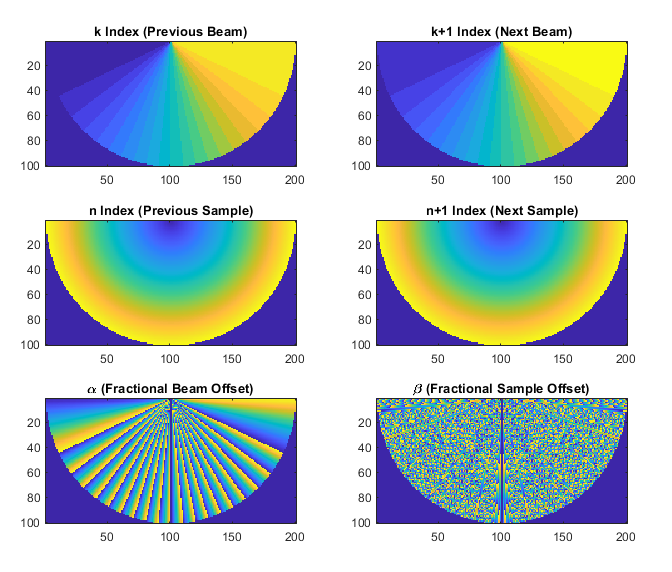
\includegraphics[width=0.8\linewidth]{figures/scan_precompute.png}
    \caption{Precomputation Plots by Image Pixel}
    \label{fig:scan_precompute}
\end{figure}

Notice that the data looks as expected.  First, we can see the previous and next beam indices sweep across the possible angles.  Additionally, the previous and next sample indices sweep through the distances.  Then, the fractional beam offset increases from zero as it gets closer to the next beam index.  The fractional sample offset does as well, though on a much smaller scale.  Thus, the precomputations were done successfully.

Next, we have three sets of synthetic data to confirm that the interpolation performs as intended.  First, we will transform and interpolate a block, as in Figure \ref{fig:scan_block}

\begin{figure}[H]
    \centering
    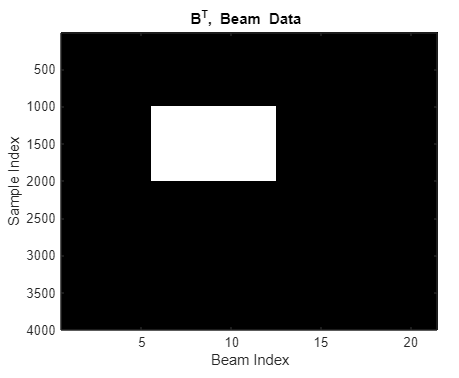
\includegraphics[width=0.5\linewidth]{figures/scan_block.png}
    \caption{Beam Data, Scan Test 1}
    \label{fig:scan_block}
\end{figure}

This beam data is successfully transformed, as can be seen in Figure \ref{fig:scan_block_out}.

\begin{figure}[H]
    \centering
    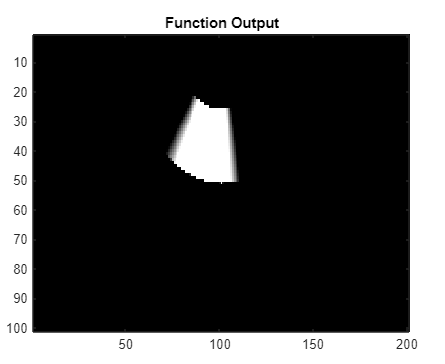
\includegraphics[width=0.5\linewidth]{figures/scan_block_out.png}
    \caption{Converted Image, Scan Test 1}
    \label{fig:scan_block_out}
\end{figure}

The next test, increasing in complexity, is with a double checkerboard, as can be seen in Figure \ref{fig:scan_checker2}.

\begin{figure}[H]
    \centering
    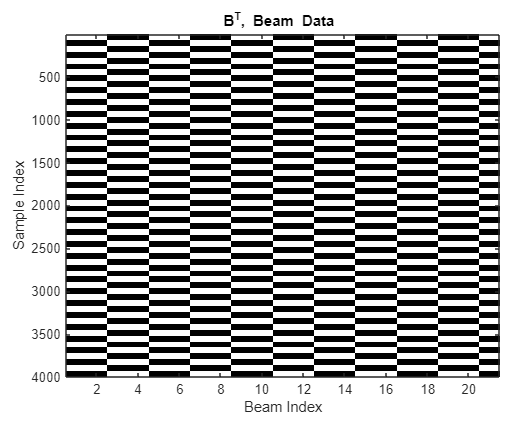
\includegraphics[width=0.5\linewidth]{figures/scan_checker2.png}
    \caption{Beam Data, Scan Test 2}
    \label{fig:scan_checker2}
\end{figure}

Again, this beam data is successfully transformed, as can be seen in Figure \ref{fig:scan_checker2_out}.

\begin{figure}[H]
    \centering
    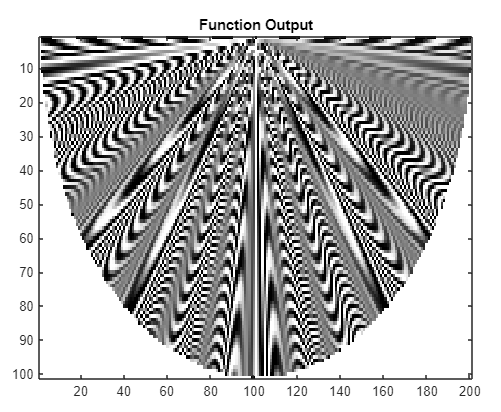
\includegraphics[width=0.5\linewidth]{figures/scan_checker2_out.png}
    \caption{Converted Image, Scan Test 2}
    \label{fig:scan_checker2_out}
\end{figure}

A third test is with a single, alternating checkerboard, as can be seen in Figure \ref{fig:scan_checker1}.

\begin{figure}[H]
    \centering
    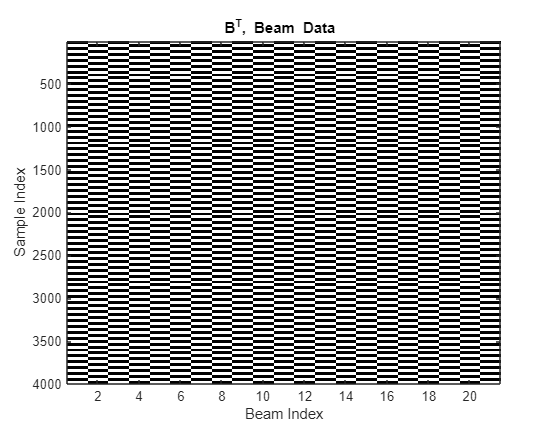
\includegraphics[width=0.5\linewidth]{figures/scan_checker1.png}
    \caption{Beam Data, Scan Test 3}
    \label{fig:scan_checker1}
\end{figure}

Again, this beam data is successfully transformed, as can be seen in Figure \ref{fig:scan_checker1_out}.

\begin{figure}[H]
    \centering
    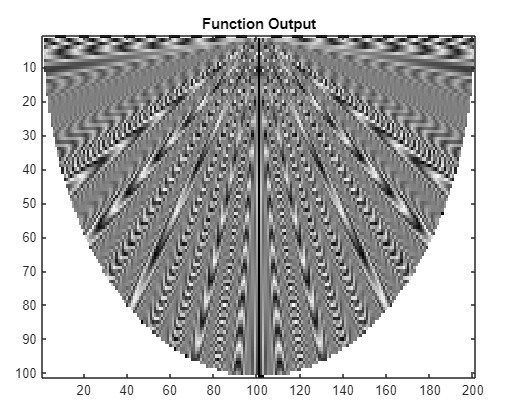
\includegraphics[width=0.5\linewidth]{figures/scan_checker1_out.png}
    \caption{Converted Image, Scan Test 3}
    \label{fig:scan_checker1_out}
\end{figure}

After conducting tests using synthetic data, we can further confirm using the real test data.  As can be seen in Figure \ref{fig:scan_real}, the system successfully interpolates real data as well.

\begin{figure}[H]
    \centering
    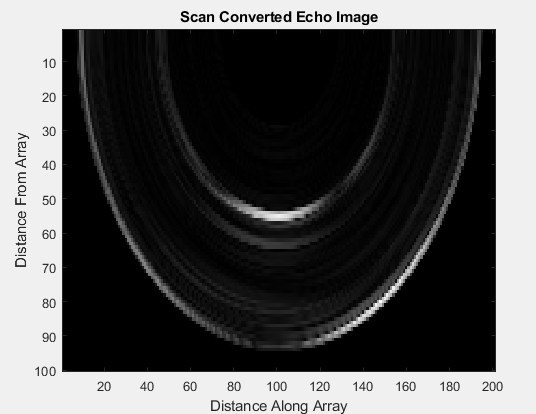
\includegraphics[width=0.5\linewidth]{figures/scan_real.png}
    \caption{Converted Image, Real Test Data}
    \label{fig:scan_real}
\end{figure}

The last aspect of the function to analyze is its timing.  Benchmarking is difficult, but here we are only comparing the newly written function to the provided \code{.p} file.  In this case, each function was timed (using \code{tic} and \code{toc}) over $10,000$ iterations, and the average runtimes can be seen in Table \ref{tab:scanConversionTime}.  The same data (the double checkerboard test pattern) was used, and the computer was in as similar a state as possible.  (Note, the provided \code{.p} function had a non-suppresed (no semicolon) line that outputted \code{max\_pixel = 10}, which needed to be suppressed using \code{evalc}, likely reducing the speed of the provided function.)

\begin{table}[H]
    \centering
    \begin{tabular}{cc}
        Function & Time ($\mu$s) \\ \hline
        Provided \code{.p} & $4002$\\
        Rewritten \code{.m} & $742.3$
    \end{tabular}
    \caption{Provided vs Rewritten Scan Conversion Performance}
    \label{tab:scanConversionTime}
\end{table}


As can be seen, the rewritten and vectorized \code{scan\_conversion.m} successfully interpolates and transforms the data into the correct format about 5 times faster than the provided function.  It is able to do this do to a substantial increase in precomputations. However, these precomputations only need to be calculated if certain configuration parameters are changed.  Thus, they are written to a file, and only incur precomputation time when necessary.  
\newpage
% !TEX root =./main.tex

\section{Block 9: Contrast/Brightness - Chen \& Stentiford}

Contrast enhancement is a critical image processing technique used to improve the visibility and
distinction of objects within an image by adjust the intensity levels of its pixels. Objects of
interest often lie within certain ranges of gray levels, which requires contrast enhancement to
highlight these important features.


\subsection{Implementation}

To implement contrast enhancement, we utilized the window/level algorithm, as seen in Figure 1.
The algorithm takes each pixel value and determines whether to supress or enhance the pixel's
brightness with threshold values.

\begin{figure}[H]
    \centering
    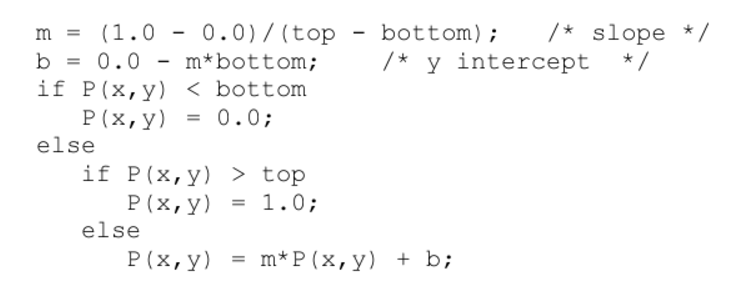
\includegraphics[width=0.5\linewidth]{figures/windowlevelalgorithm.png}
    \caption{Window/Level Algorithm}
    \label{fig:window/levelalgorithm}
\end{figure}

The contrast stage is difficult to optimize because the necessity of if-else statements precludes 
vectorization. To make the costly operation run as quickly as possible, we took the route of 
writing a native library for MATLAB in C (see contrastFix.c) to perform the operation. Not only 
are for loops written in C more performant compared to their MATLAB counterparts, C also allows 
for lower-level manipulation of data structures. In particular, 2D matrices in MATLAB require 
two index values (row and column) to access, meaning to iterate through each member of the matrix 
requires nested for loops, with the outer loop iterating through each row and the inner loop 
iterating through each member of each row. Internally, MATLAB stores all matrices as normal, 1D 
arrays (along with some metadata). As such, using C, we can iterate through each member of the matrix 
by simply looping through a normal array of numbers, meaning we only have to use one loop instead 
of a nested pair. Furthermore, C also allows specifying that certain variables should be stored in 
registers instead of memory, allowing for more efficient access of variables oft-needed for computation. 
Additionally, at the compile stage, some optimization parameters were passed to the compiler so that 
the resulting library was built with compiler code optimization, link-time optimization (where 
unnecessary function calls are bypassed), and forced usage of modern SSE (Streaming Single-Input-
Multiple-Data Extensions) instructions, which on current x86 CPUs, are more efficient that the 
standard x87 Floating Point instructions. Together, these elements ensure that the contrast stage 
ran as efficiently as possible.  
\newpage
% !TEX root =./main.tex

\section{Block 10: Persistence - Stentiford}

This stage is a bonus stage. A brief report is included nonetheless.

The persistence stage consists of an infinite impulse response filter 
implemented very simply by taking weighted averages of the current 
image and the previous image. The resulting image is then saved to be 
used as the previous image in the next iteration. The relative weights 
of the current and previous image determine how much previous images 
stick around. A higher persistence, meaning more weight is given to the 
previous image, results in better temporal noise filtering but blurs 
moving objects, while the lower persistence more clearly displays moving 
objects and the expense of more noise grain in the image.

\begin{align*}
    I_{t = n} = (1 - p)I_{new} + p*I_{t = n - 1}
\end{align*}  
\newpage
% !TEX root =./main.tex

\section{Block 11: Tracking/Velocity Estimation - Csicsila}

\subsection{Tracking}
The tracking feature add quality to the sonar project. Using an 'X' crosshair, this stage successfully follows the most prominent object as it moves across the monitor. To achieve this, the \code{xcorr2} function was used. This function takes the signal and a template and then runs a Cross-correlation algorithm to find which part of the graph most closely matches the template. This is similar to convolution. Once that is complete, the maximum point of the correlation is found and indexed to get the row and col, to overlay the crosshair on the image. 

The template is comprised of a 4x4 array filled with 1's. This template was chosen with the target in mind. The target was essentially a blob with higher values toward the center. Therefore, the template would correlate with the highest in the middle of that blob. This template plan also worked for the second object that was much longer and thinner than the first object. This is because the middle of that object still had a concentration of higher values which matched with the template.

\begin{figure}[H]
    \centering
    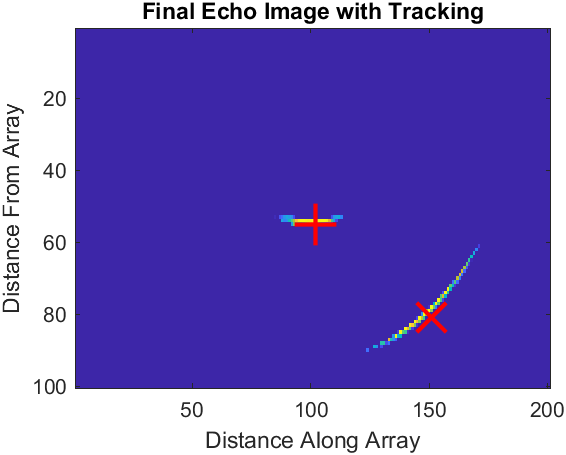
\includegraphics[width=0.5\linewidth]{figures/TrackingImage2.png}
    \caption{Final Echo Image with Tracking}
    \label{fig:TrackingImage2}
\end{figure}

Figure \ref{fig:TrackingImage2} shows the one frame where both objects are in sight with the crosshairs overlaid. The picture was colored to show the intensity around the blob better. This image also show cases the programs ability to detect two prominent images at once which will be discussed later on. 

\begin{figure}[H]
    \centering
    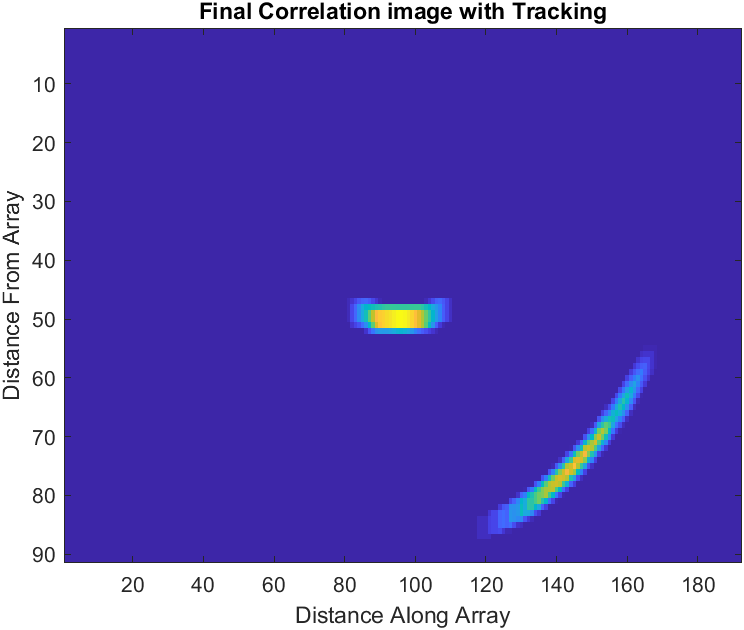
\includegraphics[width=0.5\linewidth]{figures/TrackingImage1.png}
    \caption{Final Correlation image with Tracking}
    \label{fig:TrackingImage1}
\end{figure}

Figure \ref{fig:TrackingImage1} looks very similar but shows the correlation between the template and the original signal. As you can see, the correlation made each signal thicker and more prominent. This allowed the function to better understand where the denser part of the blob was for tracking purposes.

Before testing with the live image, test data was made to ensure that it would perform correctly. The first test data utilized an array with multiple different hotspots of intensity/

\begin{figure}[H]
    \centering
    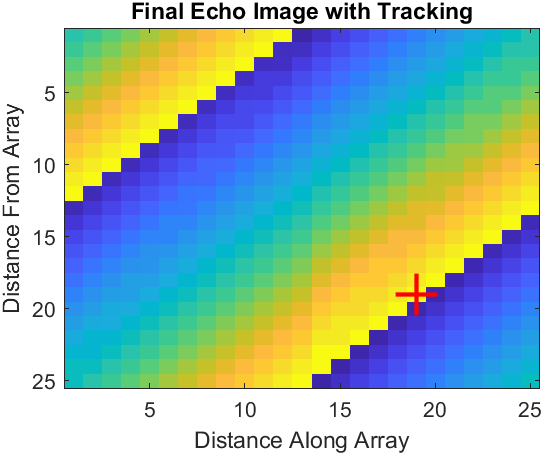
\includegraphics[width=0.5\linewidth]{figures/TrackingImage3.png}
    \caption{Test Image with Tracking}
    \label{fig:TrackingImage3}
\end{figure}

Figure \ref{fig:TrackingImage3} shows the random data with hotspots (highlighted by the lighter colors). Look what happens when the correlation with the same template is used.

\begin{figure}[H]
    \centering
    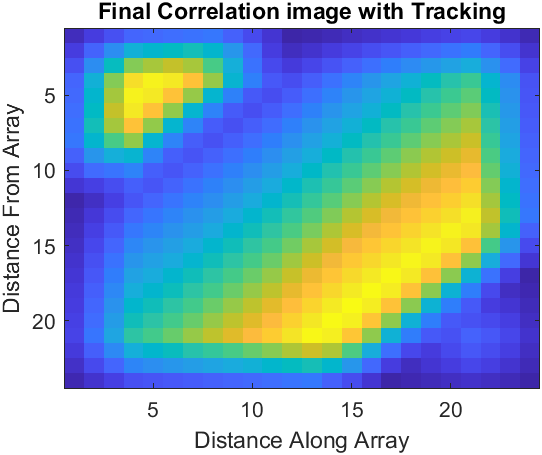
\includegraphics[width=0.5\linewidth]{figures/TrackingImage4.png}
    \caption{Test Image Correlation with Tracking}
    \label{fig:TrackingImage4}
\end{figure}

As seen in Figure \ref{fig:TrackingImage4}, the correlation was able to pick out the lower right corner as being more similar to the template. This mainly due to the lower pixel count of this image. Nevertheless, the program would work with the live image.

The next task was to try to implement tracking for two objects. This was a bit more challenging and had mild success with the live image. The problem trying to be solved was finding local maxima for the data. The first theoretical approach was to use derivatives, however this would be impractical and very slow for the size of this data. Therefore, another method was implemented. First, correlation was done in the same manner was the first tests. Then, an offset was used to zero out the values around the max value. This way, correlation could be done again without selecting the same point. 

\begin{figure}[H]
    \centering
    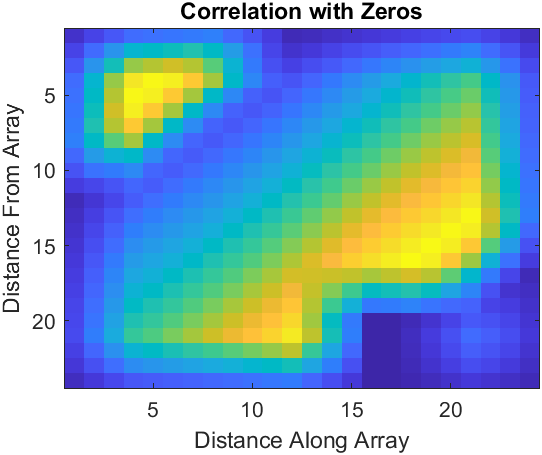
\includegraphics[width=0.5\linewidth]{figures/TrackingImage5.png}
    \caption{Test Image Correlation with Zeros}
    \label{fig:TrackingImage5}
\end{figure}

Figure \ref{fig:TrackingImage5} shows the correlation after the zeros are removed. Comparing this to \ref{fig:TrackingImage4}, there is clearly an empty spot. The zero offset could be increased to essential increase the radius in which to ignore objects around the original object.

However, an issue arose with edge cases. When setting the zeros with the offset it would sometimes set values outside the range of the array to 0 which would throw an error. To fix this, the edges of the scan were temporarily removed to avoid the error. Then the location was calculated then the edges were returned. This did not affect quality, and solved the issue.

\begin{figure}[H]
    \centering
    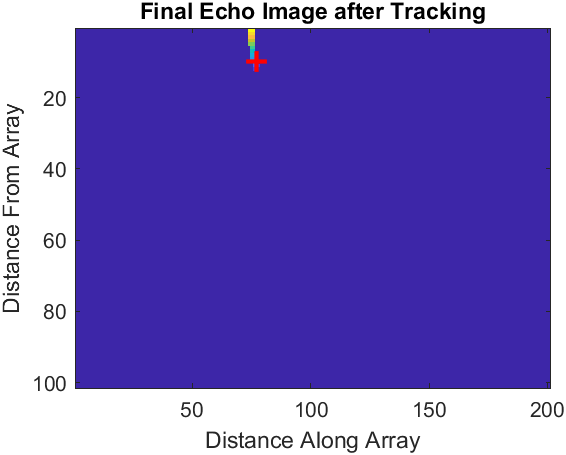
\includegraphics[width=0.5\linewidth]{figures/TrackingImage6.png}
    \caption{Image Correlation Edge Case}
    \label{fig:TrackingImage6}
\end{figure}

Figure \ref{fig:TrackingImage6} was created to test the edge cases so prove that the program could still detect images close to the edge.

\subsection{Velocity}

Velocity was extremely simple to produce. Because the tracking showed the location of the image, a simple distance equation could be used.

\begin{equation}
    d = \sqrt{(pixelPerFootRow(x_{2} - x_{1}))^{2} + pixelPerFootCol(y_{2} - y_{1})^{2}}
    \label{eq:distanceEQ}
\end{equation}

The last tricky part was figuring out the timing to get the velocity. Knowing that each scan consisted of 4000 samples, and the new up sampled sampling frequency was 200kHz, the time was found. The final step was choosing two tracked images to get the distance. An image a iteration 5 and 50 were chosen. Therefore, the final time had to be multiplied by 45 to account for the time difference between iteration.

The estimated velocity was around 2.4 ft/s.


  
\newpage
% !TEX root =./main.tex

\section{Conclusion}

For each of the five signals provided for Computer Exercise 2 (CPX 2), the processing goal was met with a filter of minimum order.  In summary, in Signal $x_1$, the louder tone was attenuated so that the quieter tone was more than $30 \unit{dB}$ greater in magnitude.  In Signal $x_8$, the secrets of extracting sunshine from cucumbers was revelaed after an attempted jamming.  In Signal $x_3$, interference from a power line in an electrocardiogram (ECG) was removed.  In Signal $x_4$, the secret to a good life according to Conan the Barbarian was revealed after another attempted jamming.  In Signal $x_7$, ten test tones were modified to be within $1 \unit{dB}$ of a specified magnitude.

For the filters for Signals $x_1$ and $x_8$, preserving linear phase was not important, and thus infinite impulse response (IIR) filters were used because they have a better magnitude response for a given order.  For Signals $x_3$ and $x_4$, preserving linear phase was important, and thus finite impulse response (FIR) filters were used.  For details on each filter, see the signal's respective section.  

Throughout this experience, I gained experience working with digital filters, in both design and application.  Additionally, I built upon my "signal hunting" skills that had been built in CPX 1 in order to understand the content of the signals, a necessary prerequisite to processing them appropriately.  I also gained more experience with audio processing in Matlab, and learned how to export to \code{.wav} files.  Additionally, I gained more experience in \LaTeX, which is always helpful.

For access to the Matlab \code{.mlx} files, source signal data, filter designer session \code{.fda} file, filter taps \code{.bin} files, and output \code{.wav} sound files, see the project's GitHub repository at \url{https://github.com/dbcometto/ece434_cpx2}.




\section*{Documentation}

I did all my own work.  I had various conversations with classmates, including C1C Csicsila and C1C Chen.  However, no changes were made based on those conversations.  Additionally, I used Google (\url{https://brainly.com/question/2233369}) to find the cucumber quote and YouTube (\url{https://www.youtube.com/watch?v=V30tyaXv6EI}) to find the Conan the Barbarian quote.  I used various resources, including overleaf.com, for Latex help.  I also used various ECG interpretation resources, including \href{https://clinical.stjohnwa.com.au/medical-library/ecg-library/introduction-overview/introduction-to-the-ecg#:~:text=Generated\%20when\%20there\%20is\%20movement,direction\%20of\%20these\%20electrical\%20impulses.&text=From\%20Atrial\%20depolarisation\%20(start\%20in,from\%20right\%20to\%20left\%20atrium.}{this article}, several YouTube videos, and several Google images of atrial fibrillation.  I also used the Mathworks website for Matlab help, for various syntax issues, and additionally for the \code{upsample} function, in an attempt to play the ECG data (until I learned that real ECGs use sonification to play the data, which makes way more sense).  I also used my notes from Math 342 Numerical Analysis and the Remez algorithm Wikipedia page.  Additionally, C1C Csicsila asked me a question regarding why it is worth finding the period in both the time domain and frequency domain, and that led me to realize I had forgot to answer several questions. 

\end{document}
